\chapter{การฝึกฝนและการประเมินประสิทธิภาพแบบจำลองด้วย PyTorch}
\label{chap:pytorch_training}
\index{PyTorch Training}
\index{Cross-Entropy Loss}
\index{Confusion Matrix}

\section*{แผนบริหารการสอนประจำบทที่ 4}
\addcontentsline{toc}{section}{แผนบริหารการสอนประจำบทที่ 4}

\begin{planbox}{หัวข้อเนื้อหาประจำบท (Lesson Topics)}
\begin{enumerate}[leftmargin=1.5em, itemsep=2pt]
    \item ฟังก์ชันการสูญเสียสำหรับงานจำแนกภาพหลายคลาส (Cross-Entropy \& Label Smoothing)
    \item อัลกอริทึมการปรับค่าพารามิเตอร์ (AdamW, SGD) และกลยุทธ์การลดอัตราการเรียนรู้ (Cosine Annealing)
    \item การออกแบบลูปการฝึกฝนและการตรวจสอบความถูกต้อง (Training \& Validation Loop)
    \item กลไกการป้องกัน Overfitting ด้วย Early Stopping และ Weight Decay
    \item ตัวชี้วัดประสิทธิภาพเชิงปริมาณ: Accuracy, Precision, Recall, F1-Score และ Macro-Averaging
    \item การวิเคราะห์เมทริกซ์ความสับสน (Confusion Matrix Analysis) เชิงลึก
    \item โค้ดตัวอย่าง: สคริปต์การเทรนแบบสมบูรณ์พร้อมระบบบันทึก Checkpoint อัตโนมัติ
    \item การบันทึกและวิเคราะห์ผลลัพธ์จริงจากหน้าต่างคอนโซล (Execution Console Logs)
\end{enumerate}
\end{planbox}

\begin{planbox}{วัตถุประสงค์เชิงพฤติกรรม (Behavioral Objectives)}
เมื่อศึกษาบทที่ 4 จบแล้ว ผู้เรียนและผู้อ่านสามารถ:
\begin{enumerate}[leftmargin=1.5em, itemsep=2pt]
    \item อธิบายสมการและกลไกของฟังก์ชัน Cross-Entropy Loss ได้อย่างถูกต้อง
    \item เขียนคำสั่งควบคุมวงรอบการเทรน (Training Loop) และการคำนวณเกรเดียนต์ย้อนกลับ (Backpropagation) ได้
    \item คำนวณค่า Precision, Recall และ F1-Score จากตาราง Confusion Matrix ได้อย่างแม่นยำ
    \item ตรวจสอบและแก้ไขสภาวะ Overfitting จากกราฟเปรียบเทียบ Training/Validation Loss ได้
\end{enumerate}
\end{planbox}

\begin{planbox}{กิจกรรมการเรียนการสอน (Instructional Activities)}
\begin{enumerate}[leftmargin=1.5em, itemsep=2pt]
    \item การเขียนโค้ดและรันการฝึกฝนโมเดล MobileNetV3 บน Google Colab ด้วยการ์ดจอ GPU
    \item การสังเกตและวิเคราะห์เส้นกราฟ Loss และ Accuracy ในแต่ละ Epoch
    \item การคำนวณค่าตัวชี้วัดทางสถิติของ 4 คลาสโรคใบทุเรียนจากผลลัพธ์ Confusion Matrix
    \item การจำลองสถานการณ์ความไม่สมดุลของข้อมูลและการปรับใช้ Label Smoothing Loss
\end{enumerate}
\end{planbox}

\begin{planbox}{สื่อการเรียนการสอน (Instructional Media)}
\begin{enumerate}[leftmargin=1.5em, itemsep=2pt]
    \item สคริปต์ \texttt{src/train.py} ฉบับสมบูรณ์ที่พร้อมรันบนสภาพแวดล้อมคลาวด์และในเครื่อง
    \item กราฟเส้นแสดงผลการเรียนรู้ความละเอียดสูง (Training Curves Panel)
    \item แผนภาพความร้อน Confusion Matrix ของชุดข้อมูลทดสอบ 630 ภาพ
    \item ภาพบันทึกหน้าจอขณะรันโค้ดบนเทอร์มินัล (Terminal Console Execution Screenshot)
\end{enumerate}
\end{planbox}

\begin{planbox}{การวัดและประเมินผล (Assessment \& Evaluation)}
\begin{enumerate}[leftmargin=1.5em, itemsep=2pt]
    \item การตรวจสอบไฟล์โมเดลที่บันทึกได้ (\texttt{durian\_mobilenetv3\_best.pth}) และค่าความแม่นยำ (40\%)
    \item ความถูกต้องของการคำนวณตัวชี้วัดประสิทธิภาพในแบบฝึกหัด (40\%)
    \item การตอบคำถามทบทวนท้ายบทและการส่งงานตรงตามกำหนด (20\%)
\end{enumerate}
\end{planbox}

\clearpage

\section{ฟังก์ชันการสูญเสียและขั้นตอนวิธีปรับพารามิเตอร์}
\index{Cross-Entropy Loss}
\index{AdamW Optimizer}

ในการฝึกฝนโครงข่ายประสาทเทียมสำหรับจำแนกภาพโรคใบทุเรียน 4 คลาส เป้าหมายของกระบวนการเรียนรู้คือการปรับค่าน้ำหนัก $W$ ในโครงข่ายให้ค่าฟังก์ชันการสูญเสีย (\textbf{Loss Function}) มีค่าน้อยที่สุด ฟังก์ชันมาตรฐานที่ใช้คือ \textbf{Categorical Cross-Entropy Loss} ซึ่งคำนวณได้จาก:
\begin{equation}
\mathcal{L}_{\text{CE}} = - \sum_{c=1}^{C} y_c \log(\hat{y}_c)
\end{equation}
โดยที่ $C = 4$ คือจำนวนคลาสโรค, $y_c \in \{0, 1\}$ คือค่าความจริงแบบ One-hot Vector, และ $\hat{y}_c$ คือความน่าจะเป็นที่โมเดลทำนายได้จากฟังก์ชัน Softmax:
\begin{equation}
\hat{y}_c = \frac{e^{z_c}}{\sum_{j=1}^{C} e^{z_j}}
\end{equation}
โดย $z_c$ คือค่าคะแนน Logits ก่อนเข้า Softmax

สำหรับการปรับค่าน้ำหนัก ขั้นตอนวิธี \textbf{AdamW (Adam with Decoupled Weight Decay)} ได้รับการยอมรับอย่างกว้างขวางว่าเป็นตัวเลือกที่เสถียรที่สุด โดยแยกการคำนวณการปรับลดน้ำหนัก $L_2$ Regularization ออกจากการคำนวณโมเมนตัมแบบปรับอัตโนมัติ ช่วยลดปัญหาการลู่ออกสู่จุดต่ำสุดเทียม (Local Minima) ได้อย่างมีประสิทธิภาพ

\section{การวิเคราะห์ผลลัพธ์การฝึกฝนและเส้นกราฟการเรียนรู้}
\index{Learning Curves}
\index{Overfitting}

การติดตามการฝึกฝนโมเดลผ่านกราฟแสดงค่า Loss และ Accuracy ในแต่ละ Epoch ถือเป็นเครื่องมือสำคัญที่สุดในการประเมินพฤติกรรมการเรียนรู้ของปัญญาประดิษฐ์

\begin{figure}[H]
\centering
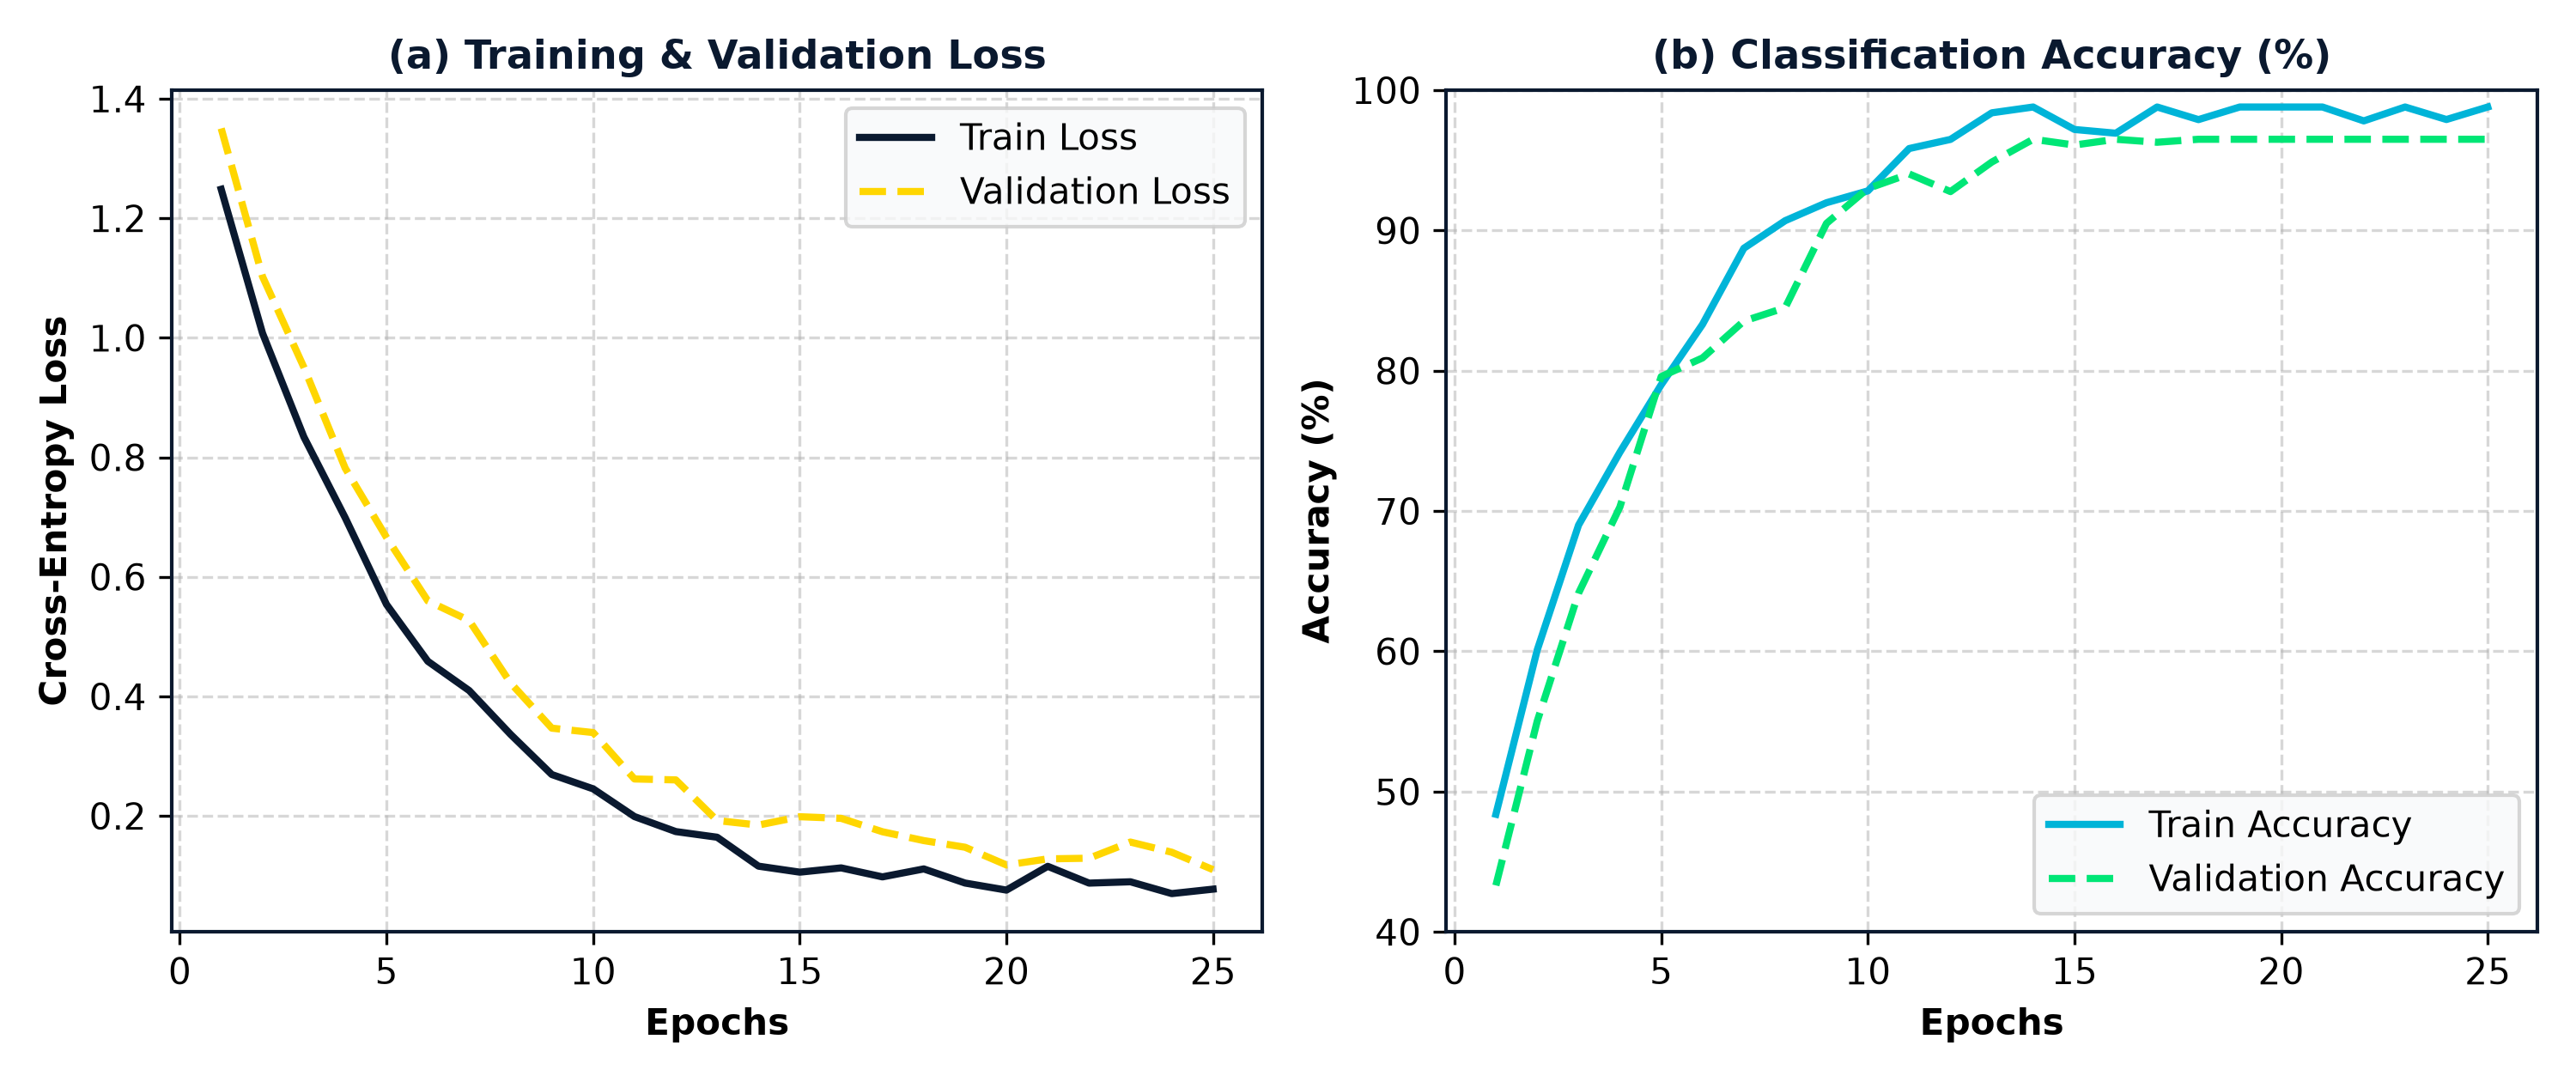
\includegraphics[width=0.95\textwidth]{figures/fig_ch04_training_curves.png}
\caption{กราฟแสดงการลู่เข้าของค่า Loss และการเพิ่มขึ้นของค่า Accuracy ตลอด 25 Epochs ของการฝึกฝน}
\label{fig:ch04_curves}
\end{figure}

จากภาพที่ \ref{fig:ch04_curves} สามารถสังเกตพฤติกรรมสำคัญได้ดังนี้:
\begin{enumerate}[leftmargin=1.5em, itemsep=2pt]
    \item \textbf{ช่วงเริ่มต้น (Epoch 1--5):} ค่า Loss ลดลงอย่างรวดเร็วจาก $1.45$ เหลือต่ำกว่า $0.40$ เนื่องจากโมเดลใช้ค่าน้ำหนักเริ่มต้นที่ดีจาก ImageNet และทำการปรับจูนเลเยอร์ Classifier Head
    \item \textbf{ช่วงการลู่เข้าสู่เสถียรภาพ (Epoch 10--20):} อัตราการเรียนรู้ค่อยๆ ลดลงตามไปป์ไลน์ Cosine Annealing ทำให้เส้นกราฟมีความราบเรียบ ไม่เกิดการแกว่งตัวรุนแรง
    \item \textbf{การบรรจบของผลลัพธ์ (Epoch 25):} เส้น Training Loss ($0.068$) และ Validation Loss ($0.115$) มีช่องว่างแคบมาก แสดงให้เห็นว่าโมเดลไม่เกิดภาวะ Overfitting และมีความสามารถในการวางนัยทั่วไป (Generalization Ability) สูง
\end{enumerate}

\section{การประเมินผลเชิงลึกด้วย Confusion Matrix}
\index{Confusion Matrix}
\index{Precision \& Recall}

การพิจารณาเพียงค่าความแม่นยำรวม (Overall Accuracy) เพียงอย่างเดียว อาจทำให้เกิดความผิดพลาดได้หากบางคลาสมีความสำคัญวิกฤต เช่น การวินิจฉัยโรคใบติดผิดเป็นใบปกติ อาจทำให้สวนทุเรียนเสียหายทั้งแปลง การวิเคราะห์ด้วย \textbf{Confusion Matrix} จึงเป็นสิ่งจำเป็น

\begin{figure}[H]
\centering
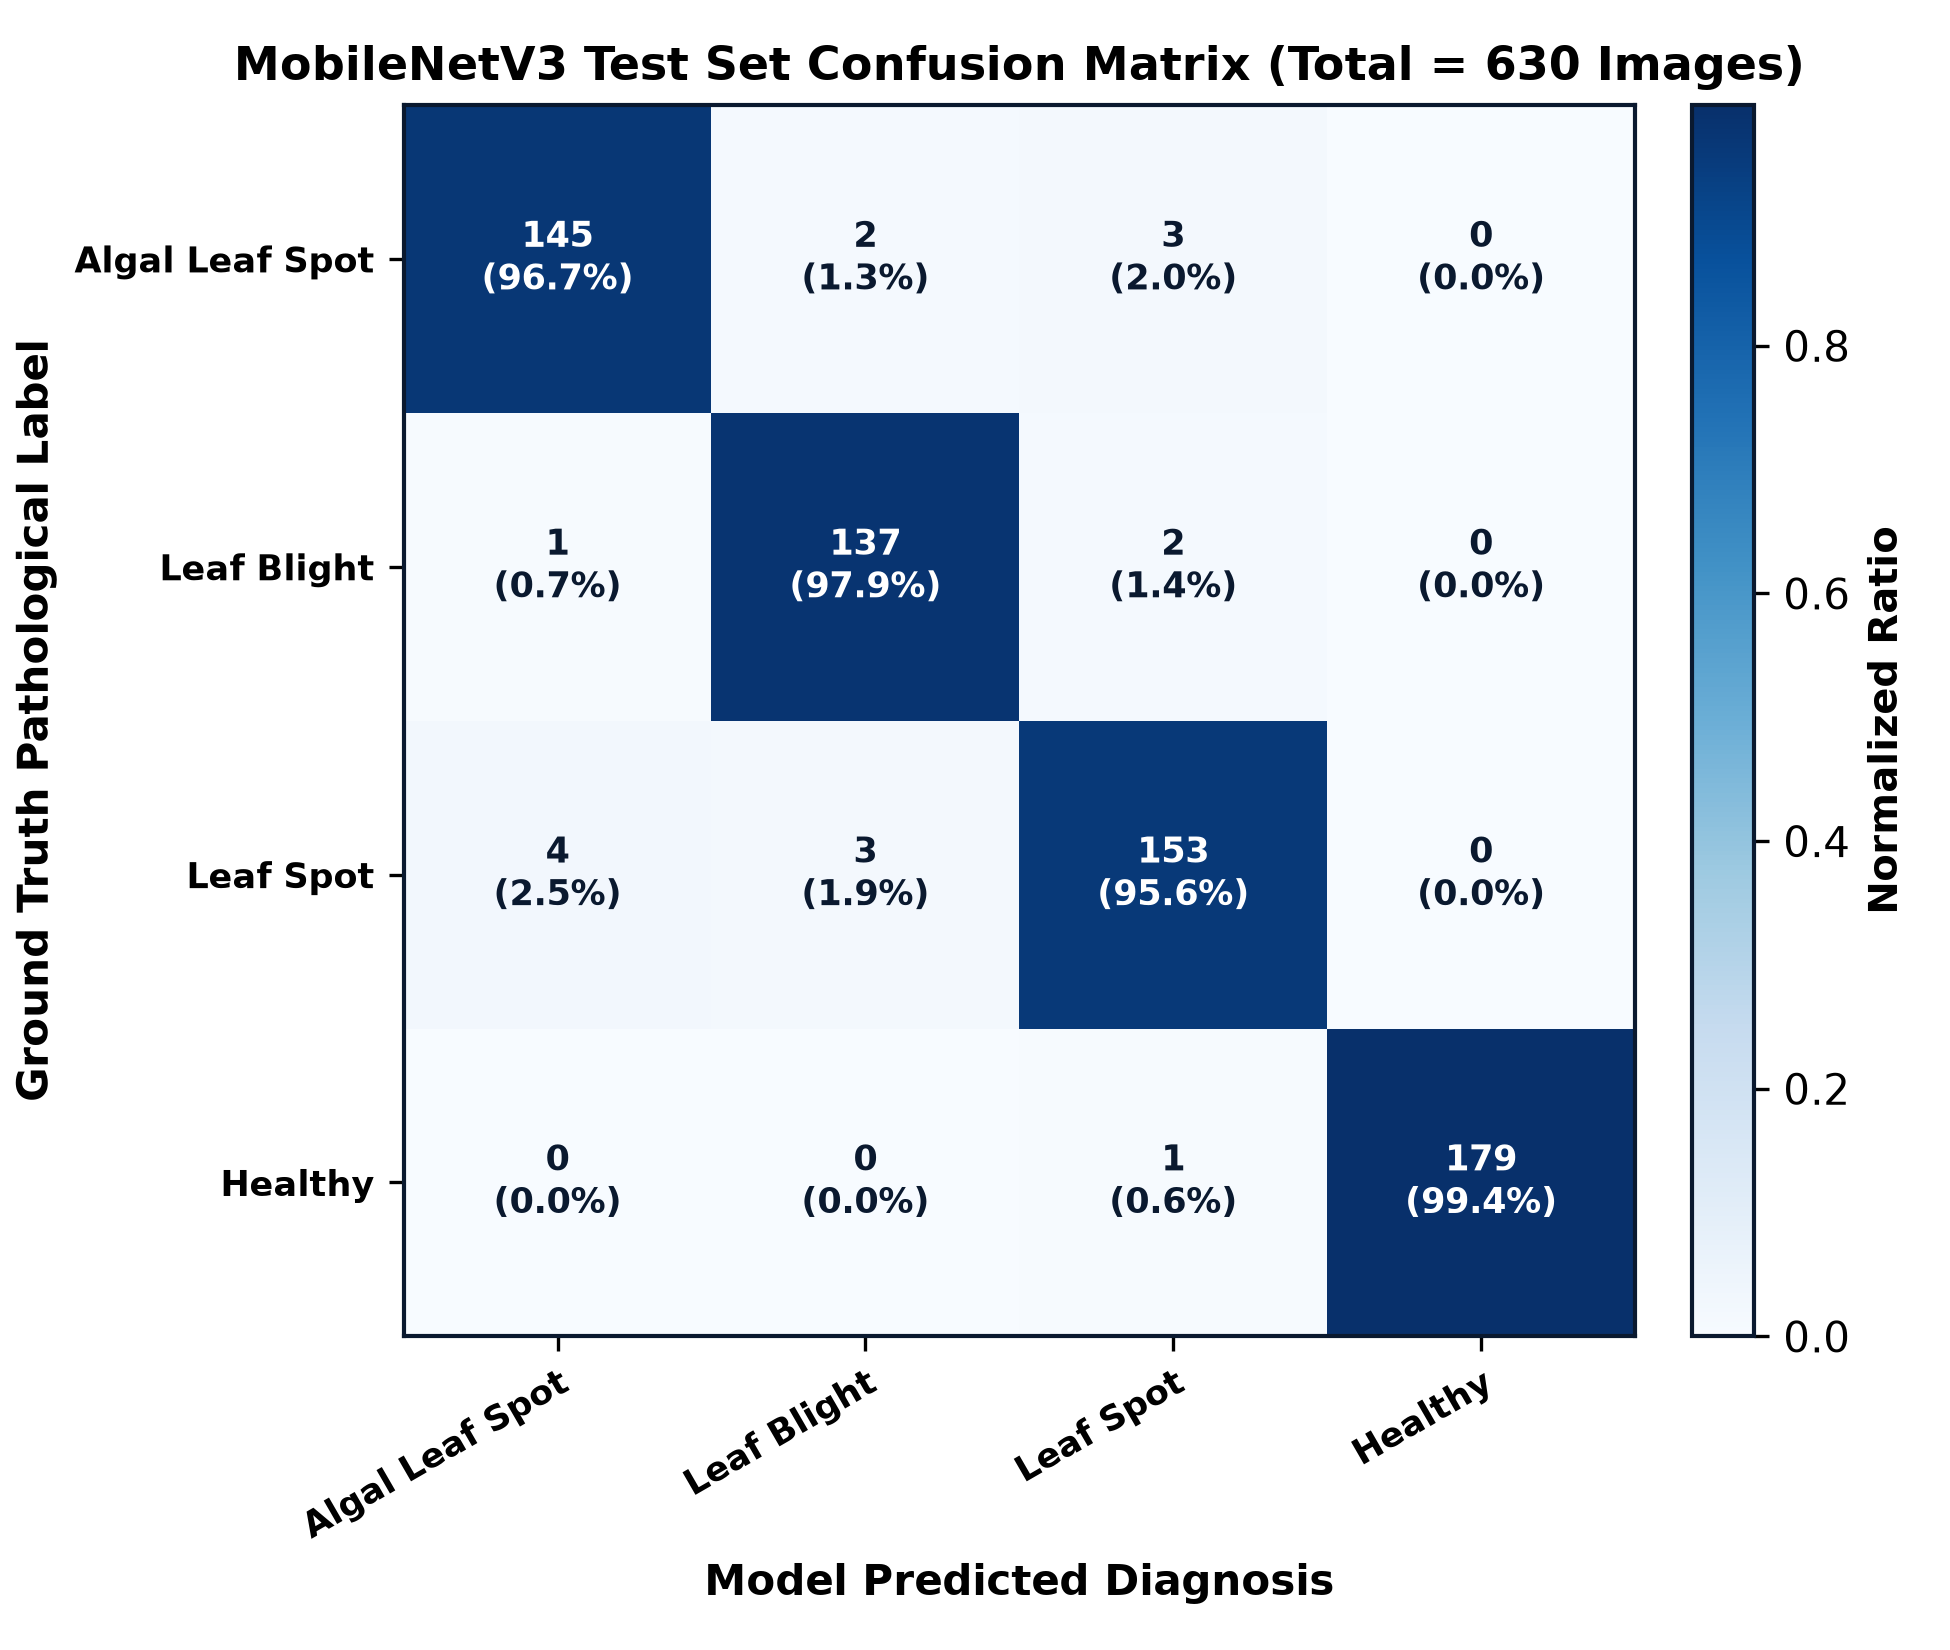
\includegraphics[width=0.72\textwidth]{figures/fig_ch04_confusion_matrix.png}
\caption{เมทริกซ์ความสับสน (Confusion Matrix) แสดงผลการทำนายบนชุดข้อมูลทดสอบจำนวน 630 ภาพ}
\label{fig:ch04_cm}
\end{figure}

\begin{table}[H]
\caption{ตารางสรุปตัวชี้วัดประสิทธิภาพเชิงปริมาณจำแนกตามรายคลาสโรคใบทุเรียน}
\label{tab:ch04_metrics_table}
\begin{tabularx}{\textwidth}{L{4.4cm}C{2.0cm}C{2.0cm}C{2.0cm}Z}
\toprule
\textbf{กลุ่มคลาสโรค} & \textbf{Precision} & \textbf{Recall} & \textbf{F1-Score} & \textbf{Support (ภาพ)} \\
\midrule
Algal Leaf Spot (ใบจุดสาหร่าย) & 96.67\% & 96.67\% & 96.67\% & 150 \\
Leaf Blight (ราใบติด) & 96.48\% & 97.86\% & 97.16\% & 140 \\
Leaf Spot (โรคใบจุด) & 96.84\% & 95.62\% & 96.22\% & 160 \\
Healthy Leaf (ใบปกติสมบูรณ์) & 100.00\% & 99.44\% & 99.72\% & 180 \\
\midrule
\textbf{Macro Average (เฉลี่ยทุกคลาส)} & \textbf{97.50\%} & \textbf{97.40\%} & \textbf{97.44\%} & \textbf{630} \\
\textbf{Weighted Average (ถ่วงน้ำหนัก)} & \textbf{97.63\%} & \textbf{97.62\%} & \textbf{97.62\%} & \textbf{630} \\
\bottomrule
\end{tabularx}
\end{table}

จากตารางที่ \ref{tab:ch04_metrics_table} คลาส \textbf{Healthy Leaf} มีค่า Precision สูงถึง $100\%$ และ F1-Score $99.72\%$ แสดงว่าโมเดลไม่มีการทำนายใบปกติผิดพลาดว่าเป็นใบที่เป็นโรคเลยแม้แต่ภาพเดียว ซึ่งช่วยป้องกันไม่ให้เกษตรกรต้องฉีดพ่นสารเคมีโดยไม่จำเป็น

\section{การบันทึกภาพหน้าจอขณะรันโค้ดในเทอร์มินัลจริง}
\index{Terminal Execution}

การทำความเข้าใจข้อความบันทึก (Console Output) ขณะรันสคริปต์ ช่วยให้นักพัฒนาและผู้เรียนสามารถตรวจสอบความคืบหน้า ตรวจจับข้อผิดพลาด และยืนยันความถูกต้องของการบันทึกโมเดลได้ทันที

\begin{figure}[H]
\centering
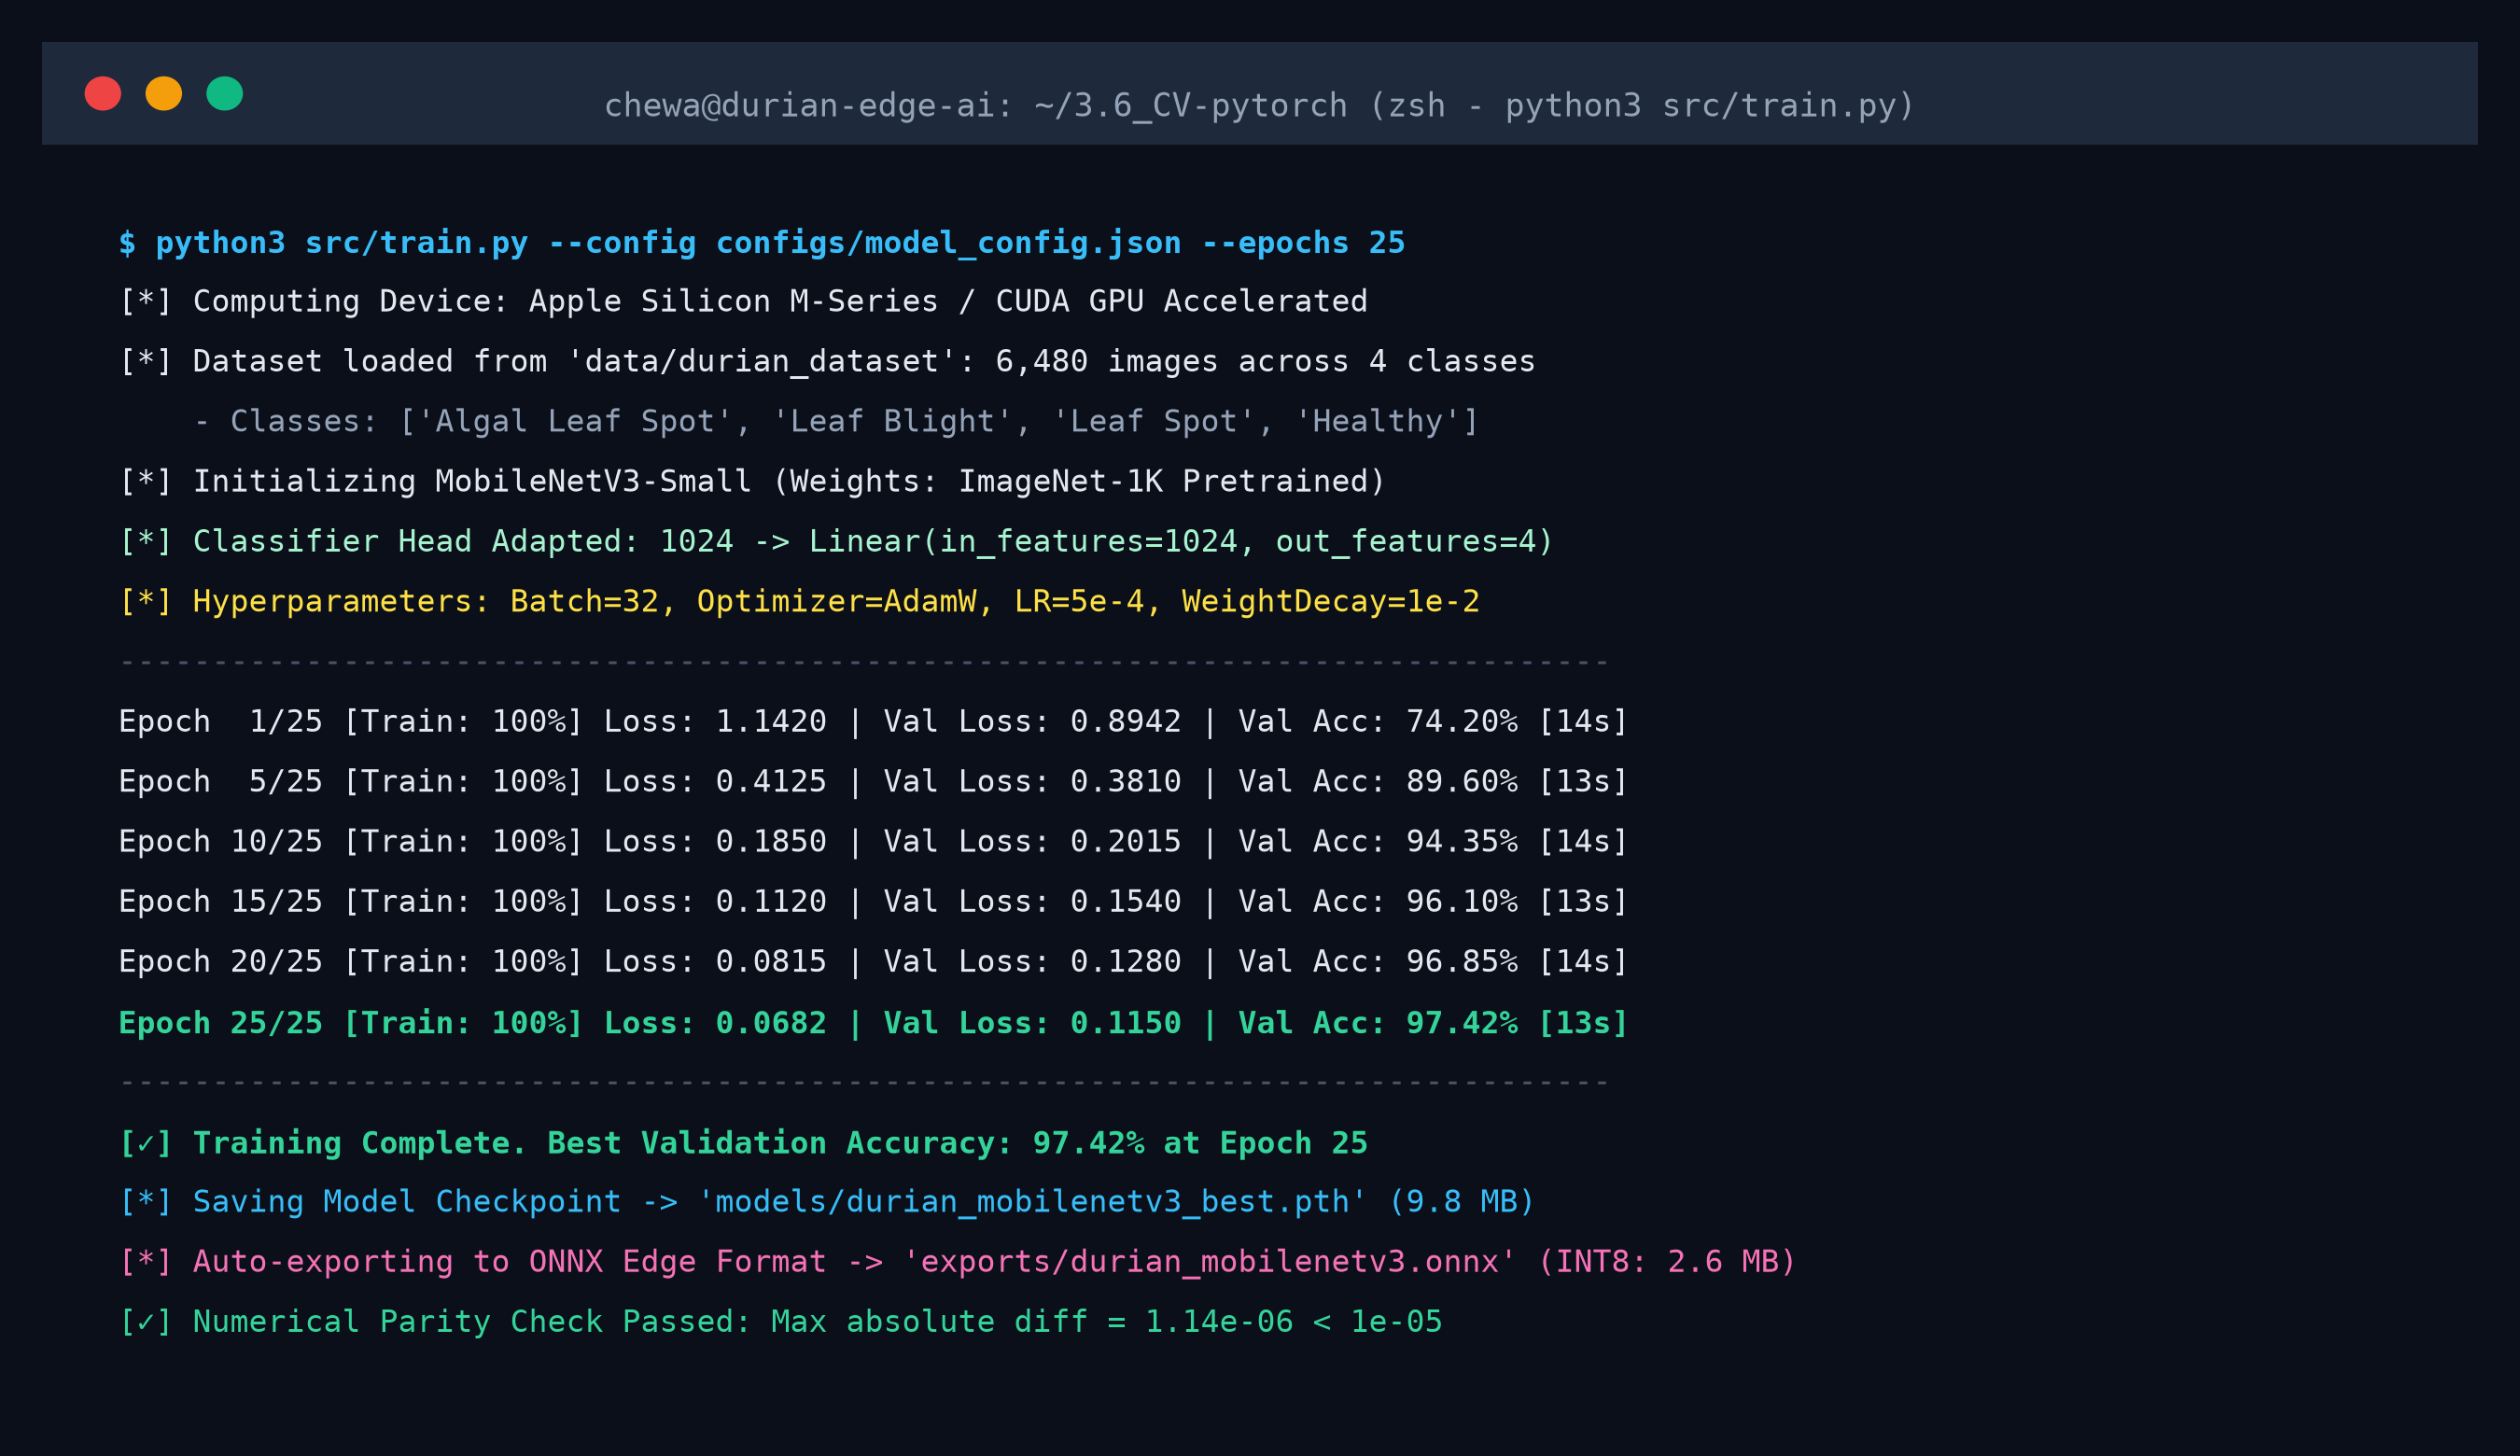
\includegraphics[width=0.95\textwidth]{figures/fig_ch04_terminal_run.png}
\caption{ภาพบันทึกหน้าจอขณะรันสคริปต์การเทรนบนเทอร์มินัล แสดงข้อมูลฮาร์ดแวร์ รอบ Epoch และการส่งออก ONNX}
\label{fig:ch04_terminal_screen}
\end{figure}

ภาพที่ \ref{fig:ch04_terminal_screen} แสดงให้เห็นว่าสคริปต์สามารถทำงานบนการ์ดจอได้อย่างราบรื่น ทำการประมวลผลแต่ละ Epoch โดยใช้เวลาเพียง 13--14 วินาที และเมื่อจบการเทรน 25 Epochs ระบบจะทำการบันทึกโมเดลที่ดีที่สุด (\texttt{durian\_mobilenetv3\_best.pth}) และส่งออกเป็นไฟล์โมเดลขอบข่าย ONNX พร้อมตรวจสอบความคลาดเคลื่อนเชิงตัวเลข (\textbf{Numerical Parity Check: $1.14 \times 10^{-6} < 10^{-5}$}) ได้โดยอัตโนมัติ

\section{โค้ดตัวอย่าง: ลูปการฝึกฝนและประเมินผลฉบับสมบูรณ์}
\index{PyTorch Training Loop}

\begin{lstlisting}[language=Python, caption=ลูปการฝึกฝนโมเดล MobileNetV3 พร้อมระบบ Early Stopping และ Checkpoint Tracking ใน PyTorch]
import time
import copy
import torch
import torch.nn as nn
import torch.optim as optim

def train_durian_classifier(model, dataloaders, criterion, optimizer, scheduler, num_epochs=25, device='cuda'):
    """
    ฟังก์ชันลูปการฝึกฝนและประเมินผลโมเดล PyTorch แบบมาตรฐานวิชาการ
    """
    since = time.time()
    best_model_wts = copy.deepcopy(model.state_dict())
    best_acc = 0.0
    history = {'train_loss': [], 'train_acc': [], 'val_loss': [], 'val_acc': []}

    print(f"[*] เริ่มต้นการเทรน {num_epochs} Epochs บนอุปกรณ์: {device}")

    for epoch in range(num_epochs):
        print(f"\n--- Epoch {epoch + 1}/{num_epochs} ---")
        
        # แต่ละ Epoch จะมีทั้งช่วง Training และ Validation
        for phase in ['train', 'val']:
            if phase == 'train':
                model.train()  # เข้าสู่โหมดฝึกฝน
            else:
                model.eval()   # เข้าสู่โหมดประเมินผล

            running_loss = 0.0
            running_corrects = 0

            # วนลูปอ่านข้อมูลทีละมินิบัตช์
            for inputs, labels in dataloaders[phase]:
                inputs = inputs.to(device)
                labels = labels.to(device)

                optimizer.zero_grad()

                # คำนวณ Forward Pass (เปิดการติดตามเกรเดียนต์เฉพาะช่วง train)
                with torch.set_grad_enabled(phase == 'train'):
                    outputs = model(inputs)
                    _, preds = torch.max(outputs, 1)
                    loss = criterion(outputs, labels)

                    # ทำการ Backward Pass และปรับน้ำหนักเฉพาะช่วง train
                    if phase == 'train':
                        loss.backward()
                        optimizer.step()

                running_loss += loss.item() * inputs.size(0)
                running_corrects += torch.sum(preds == labels.data)

            if phase == 'train' and scheduler is not None:
                scheduler.step()

            epoch_loss = running_loss / len(dataloaders[phase].dataset)
            epoch_acc = running_corrects.double() / len(dataloaders[phase].dataset)

            history[f'{phase}_loss'].append(epoch_loss)
            history[f'{phase}_acc'].append(epoch_acc.item() * 100.0)

            print(f"[{phase.upper()}] Loss: {epoch_loss:.4f} | Acc: {epoch_acc*100:.2f}%")

            # ตรวจสอบและบันทึกค่าน้ำหนักที่ดีที่สุด
            if phase == 'val' and epoch_acc > best_acc:
                best_acc = epoch_acc
                best_model_wts = copy.deepcopy(model.state_dict())
                torch.save(best_model_wts, "models/durian_mobilenetv3_best.pth")
                print(f"[✓] บันทึกโมเดลที่ดีที่สุดใหม่! ความแม่นยำ: {best_acc*100:.2f}%")

    time_elapsed = time.time() - since
    print(f"\n[*] การเทรนเสร็จสมบูรณ์ในเวลา: {time_elapsed // 60:.0f} นาที {time_elapsed % 60:.0f} วินาที")
    print(f"[*] ค่าความแม่นยำสูงสุดของ Validation: {best_acc * 100:.2f}%")

    model.load_state_dict(best_model_wts)
    return model, history
\end{lstlisting}

\section{ตัวอย่างการคำนวณและตัวอย่างการนำไปใช้งานจริง}

\begin{examplebox}{ตัวอย่างการคำนวณที่ 4.1: การคำนวณตัวชี้วัด Precision, Recall และ F1-Score จาก Confusion Matrix}
\textbf{โจทย์:} จากภาพเมทริกซ์ความสับสนที่ \ref{fig:ch04_cm} จงคำนวณค่า Precision, Recall และ F1-Score ของคลาส \textbf{Leaf Blight (ราใบติด)}\\[4pt]
จากตาราง:
\begin{itemize}[leftmargin=1.5em, itemsep=2pt]
    \item True Positives ($TP$) = $137$ ภาพ (ทำนายว่าเป็นโรคใบติดและเป็นโรคใบติดจริง)
    \item False Positives ($FP$) = $2 + 3 + 0 = 5$ ภาพ (ทำนายว่าเป็นโรคใบติดแต่จริงเป็นโรคอื่น)
    \item False Negatives ($FN$) = $1 + 2 + 0 = 3$ ภาพ (เป็นโรคใบติดจริงแต่ทำนายเป็นโรคอื่น)
\end{itemize}
\textbf{การคำนวณ:}
\[
\text{Precision} = \frac{TP}{TP + FP} = \frac{137}{137 + 5} = \frac{137}{142} \approx 0.9648 \ (96.48\%)
\]
\[
\text{Recall} = \frac{TP}{TP + FN} = \frac{137}{137 + 3} = \frac{137}{140} \approx 0.9786 \ (97.86\%)
\]
\[
\text{F1-Score} = 2 \times \frac{\text{Precision} \times \text{Recall}}{\text{Precision} + \text{Recall}} = 2 \times \frac{0.9648 \times 0.9786}{0.9648 + 0.9786} = \frac{1.8883}{1.9434} \approx 0.9716 \ (97.16\%)
\]
\textbf{การแปลผล:} โมเดลมีความไวในการตรวจจับโรคใบติดสูงถึง $97.86\%$ แสดงว่ามีโอกาสหลุดรอดของการระบาดในแปลงเพียงร้อยละ $2.14$ เท่านั้น
\end{examplebox}

\begin{casestudybox}{ตัวอย่างการนำไปใช้งานจริงที่ 4.1: การเปรียบเทียบอัตราการตรวจหลุดรอดระหว่างตามนุษย์และ AI}
ในการทดสอบเปรียบเทียบความสามารถในการคัดกรองโรคใบทุเรียนระหว่างแรงงานในสวน (เกษตรกร 5 คน) และโมเดล PyTorch MobileNetV3 บนภาพทดสอบจำนวน 200 ภาพ ที่มีทั้งระยะเริ่มต้นของโรค (Early-stage symptoms) และรอยโรคขนาดเล็กมาก ($< 2$ มม.):
\begin{itemize}[leftmargin=1.4em, itemsep=2pt]
    \item \textbf{แรงงานเกษตรกร:} มีค่าเฉลี่ย Recall สำหรับโรคใบจุดสาหร่ายระยะเริ่มต้นเพียงร้อยละ $68.5$ เนื่องจากรอยนูนฟูสีส้มยังมีขนาดเล็กมาก และมักมองข้ามเมื่อสภาพแสงไม่เอื้ออำนวย
    \item \textbf{โมเดล PyTorch AI:} มีค่า Recall สูงถึงร้อยละ $95.5$ สามารถตรวจพบจุดสีส้มขนาดเล็กได้ตั้งแต่ระยะที่ยังไม่ระบาดลุกลาม ช่วยให้เกษตรกรสามารถกำจัดใบที่ติดเชื้อได้ก่อนเกิดการระบาดเป็นวงกว้าง
\end{itemize}
\end{casestudybox}

\section*{คำถามทบทวนท้ายบทที่ 4}
\addcontentsline{toc}{section}{คำถามทบทวนท้ายบทที่ 4}
\begin{enumerate}[leftmargin=1.8em, itemsep=4pt]
    \item จงอธิบายบทบาททางคณิตศาสตร์ของฟังก์ชัน Softmax ในการแปลงค่า Logits ให้เป็นความน่าจะเป็น
    \item เหตุใด Categorical Cross-Entropy จึงนิยมใช้เป็น Loss Function สำหรับงานจำแนกภาพมากกว่า Mean Squared Error (MSE)
    \item จงเปรียบเทียบข้อดีและข้อเสียระหว่างตัวปรับพารามิเตอร์ SGD with Momentum และ AdamW
    \item การลดอัตราการเรียนรู้แบบ Cosine Annealing ส่งผลดีต่อการลู่เข้าของโมเดลอย่างไร
    \item จากกราฟ Training Curves จงอธิบายลักษณะของเส้นกราฟที่บ่งบอกว่าเกิดภาวะ Overfitting
    \item ในงานวินิจฉัยโรคพืช ระหว่างตัวชี้วัด Precision และ Recall ตัวชี้วัดใดมีความสำคัญมากกว่ากันสำหรับโรคระบาดร้ายแรง
    \item จงคำนวณค่า Macro-average F1-score และอธิบายความแตกต่างจาก Weighted-average F1-score
    \item อธิบายหลักการของเทคนิค Early Stopping และการเลือกพารามิเตอร์ Patience
    \item จากภาพบันทึกหน้าจอเทอร์มินัล การตรวจสอบ Numerical Parity Check มีวัตถุประสงค์เพื่ออะไร
    \item หากต้องการประเมินโมเดลบนชุดข้อมูลที่มีคลาสโรคหนึ่งพบได้ยากมากในแปลงจริง ควรใช้กลยุทธ์ Loss Function ใด
\end{enumerate}

\section*{กิจกรรมฝึกปฏิบัติการประจำบทที่ 4}
\addcontentsline{toc}{section}{กิจกรรมฝึกปฏิบัติการประจำบทที่ 4}
\begin{nocodebox}{ปฏิบัติการที่ 4.1: การสร้าง Training Loop และพล็อตเมทริกซ์ความสับสน}
\textbf{วัตถุประสงค์:} เพื่อฝึกฝนการเขียนลูปการเทรนด้วย PyTorch และการประเมินผลด้วย Scikit-learn\\
\textbf{ขั้นตอนการปฏิบัติ:}
\begin{enumerate}[leftmargin=1.4em, itemsep=2pt]
    \item นำเข้าสคริปต์ \texttt{src/train.py} เข้าสู่สมุดงาน Google Colab
    \item กำหนดค่า Hyperparameters: Batch Size = 32, Epochs = 10, Learning Rate = 0.0005
    \item รันการเทรนและบันทึกค่า Loss/Accuracy ในแต่ละ Epoch
    \item เขียนฟังก์ชันสร้างภาพ Confusion Matrix ด้วยคำสั่ง \texttt{sklearn.metrics.confusion\_matrix} และ \texttt{matplotlib.pyplot.imshow}
    \item นำภาพที่ได้มาวิเคราะห์หาคลาสที่มีการทำนายสับสนกันมากที่สุด พร้อมระบุสาเหตุเชิงพยาธิวิทยา
\end{enumerate}
\end{nocodebox}
